\documentclass{article}
\usepackage{graphicx} % Load the graphicx package
\usepackage{amsmath} % Required for math symbols like \frac


\begin{document}
\title{Exercício 7} 
\author{Arthur Felipe Reis Souza}
\date{\today}
\maketitle

\section{Introduction}

Os conjuntos de dados que serão avaliados são, respectivamente, Breast Cancer e Statlog. Ambos os datasets contém informações e características que irão contribuir parcialmente para predizer se uma pessoa tem ou não tem alguma doença. Para isso, serão utilizados modelos de redes neurais do tipo ELM (Extreme Learning Machine) ou RBF (Radial Basis Function).

\subsection{StatLog}

O dataset StatLog contém várias características e informações de 270 pacientes, essas características serão utilizadas para predizer se os pacientes de teste tem ou não doença de coração. Primeiramente, o conjunto de dados foi pré processado, ou seja, as colunas que continham características discrepantes e que atrapalhavam a convergência da rede foram transformadas. Foi utilizada uma função da biblioteca skilearn que desloca a função para a origem e a escala para  ter um desvio padrão de 1 : 

\[ \hspace{1cm} x_i = \frac{x - \mu}{\sigma} \]


\vspace{10pt}

Com os dados pré processados, o algoritmo KMeans com K = 10 foi utilizado, portanto terá 10 funções radiais na camada intermediária da rede RBF.

\vspace{10pt}

\begin{center}

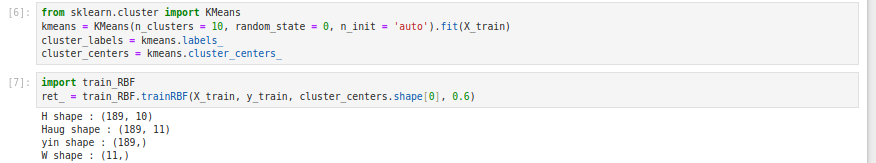
\includegraphics[height=1in]{/home/arthur/Desktop/RNA_BRAGA/RBF/KMeans_statlog.png}
    
\end{center}

\vspace{10pt}

Após treinar a rede, um conjunto de 81 dados foram utilizados para teste. Foram criados vários modelos, e cada um foi testado obtendo a acurácia do mesmo. Esse algoritmo é chamado de Grid Search Cross-Validation, e tem por objetivo, dado um conjunto e possíveis parâmetros, selecionar o modelo que teve o melhor desempenho sobre os dados de teste. Portanto, a ideia do Grid Search aqui foi de encontrar o melhor valor de neurônios radiais para os quais uma boa performance em uma dada métrica de validação é satisfeita.

\vspace{10pt}

\begin{center}

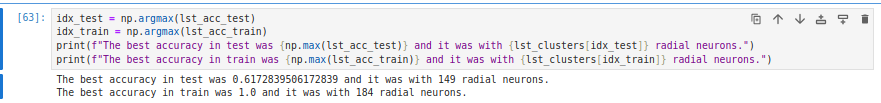
\includegraphics[height=0.5in]{/home/arthur/Desktop/RNA_BRAGA/RBF/performance.png}
    
\end{center}

\vspace{10pt}

Analisando o resultado acima, é possível afirmar que 149 neurônios radiais nos darão uma melhor performance dado um conjunto de dados de teste. Outro ponto é, utilizando mais neurônios radiais, o modelo terá uma acurácia de 100\% sobre os dados de treino, mas não generalizará bem para os dados de teste. Isso acontecerá porque o modelo neuronal do tipo RBF, com uma grande quantidade de neurônios na camada intermediária, tenderá a sobreajustar (overfitting) aos dados.

\vspace{10pt}


\subsection{Breast Cancer}

O dataset Breast Cancer contém várias características e informações de 699 pacientes, essas características serão utilizadas para predizer se os pacientes de teste tem um tumor maligno ou benigno. Primeiramente, o conjunto de dados foi pré processado, ou seja, as colunas que continham características discrepantes e que atrapalhavam a convergência da rede foram transformadas.


\vspace{10pt}

Com os dados pré processados, o algoritmo KMeans com K = 10 foi utilizado, portanto terá 10 funções radiais na camada intermediária da rede RBF.

\vspace{10pt}

Após treinar a rede, um conjunto de 210 dados foram utilizados para teste. Foram criados vários modelos, e cada um foi testado obtendo a acurácia do mesmo. Esse método é chamado de Grid Search Cross-Validation, e tem por objetivo, dado um conjunto e possíveis parâmetros, selecionar o modelo que teve o melhor desempenho sobre os dados de teste. Portanto, a ideia do Grid Search aqui foi de encontrar o melhor valor de neurônios radiais para os quais uma boa performance em uma dada métrica de validação é satisfeita.

\vspace{10pt}

\begin{center}

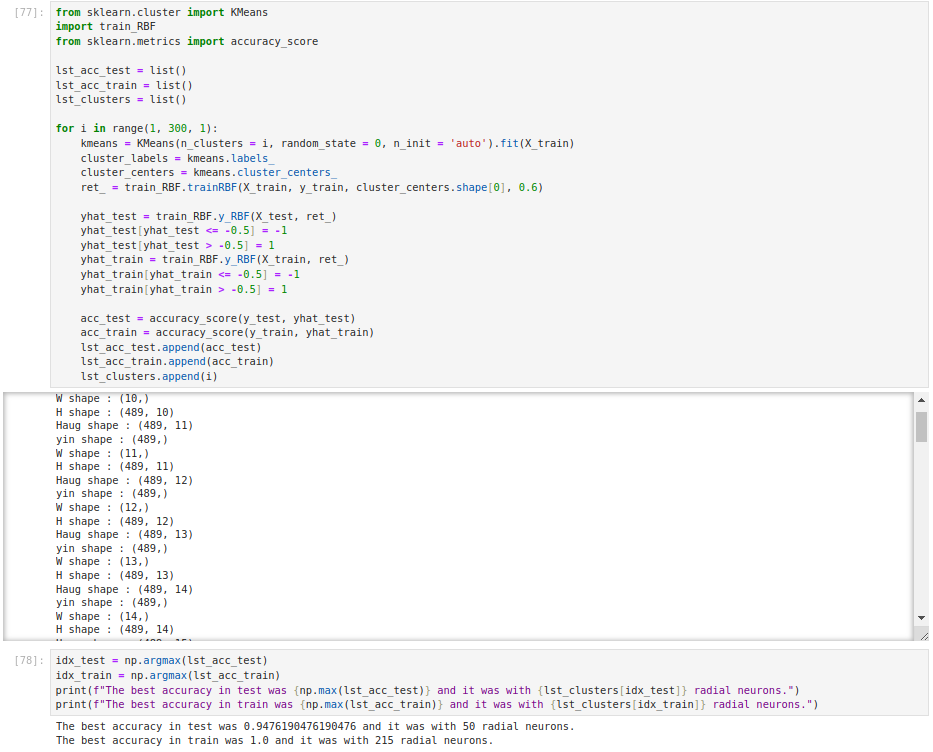
\includegraphics[height=3.5in]{/home/arthur/Desktop/RNA_BRAGA/ex08/grid_search_breast.png}
        
\end{center}

\vspace{10pt}

Analisando o resultado acima, é possível afirmar que 50 neurônios radiais nos darão uma melhor performance dado um conjunto de dados de teste. Usando 215 neuronios na camada intermediária, a acurácia nos dados de treino é de 100\%. O segundo resultado é esperado, considerando-se que um grande número de neurônios na camada intermediária tenderá o modelo à um overfitting.

\vspace{10pt}



\section{Centros aleatórios}

\vspace{10pt}

A lógica para escolher os centros e os raios aleatórios são : os pontos centrais das funções radiais serão exatamente o primeiro e o terceiro quartile. O primeiro quartile é a mediana do conjunto abaixo da mediana, enquanto o terceiro quartile é a mediana do conjunto acima da mediana. O raio será a metade da distância entre os quartiles. Após realizar o treinamento da rede neuronal RBF com esses valores de centro, foram obtidos os resultados abaixo : 

\vspace{10pt}

\subsection{StatLog}

\vspace{10pt}

Para o dataset statlog utilizando os 2 centros sendo, respectivamente o primeiro e o terceiro quartile, obtemos a acurácia média e o erro (desvio padrão): 

\begin{center}

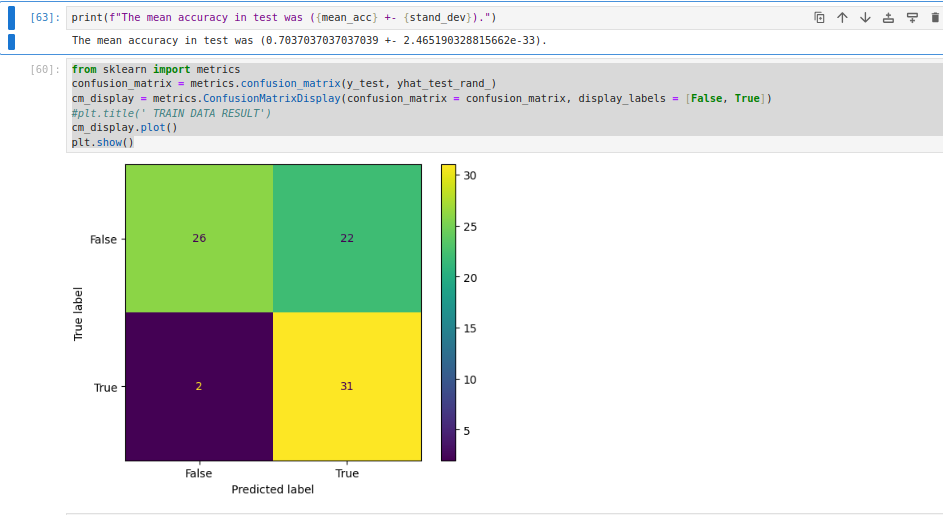
\includegraphics[height=2.5in]{/home/arthur/Desktop/RNA_BRAGA/ex08/statlog_mean_acc.png}
            
\end{center}

\vspace{10pt}

\subsection{Breast Cancer}

\vspace{10pt}

Para o Breast statlog utilizando os 2 centros sendo, respectivamente o primeiro e o terceiro quartile, obtemos a acurácia média e o erro (desvio padrão): 

\vspace{10pt}

\begin{center}

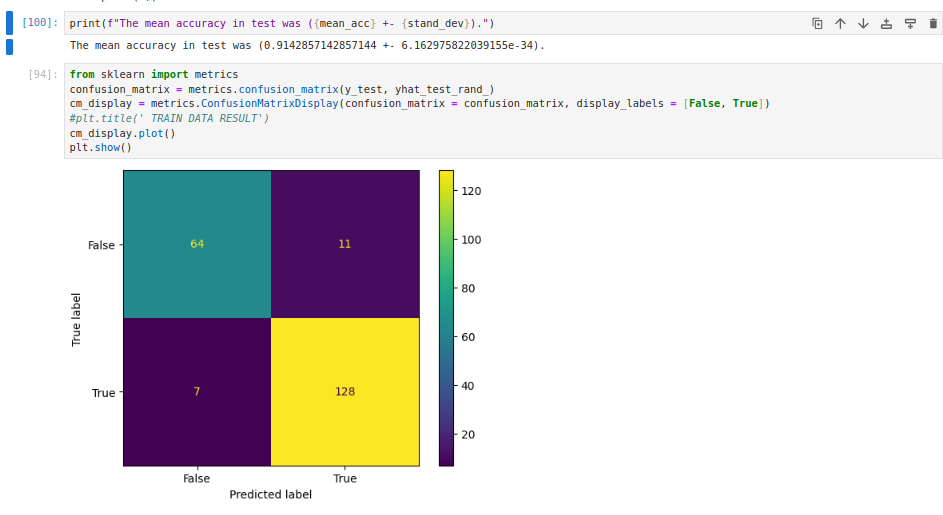
\includegraphics[height=2.5in]{/home/arthur/Desktop/RNA_BRAGA/ex08/breast_cancer_mean_acc.png}
            
\end{center}

\vspace{10pt}



\section{Statlog}
\vspace{10pt}

Por fim, após realizar em um Grid Search o teste de N valores de K clusters, foram obtidos as seguintes aproximações em relação ao modelo com funções radiais arbitrárias : 

\vspace{10pt}

\subsection{Statlog}

\vspace{10pt}


\begin{center}

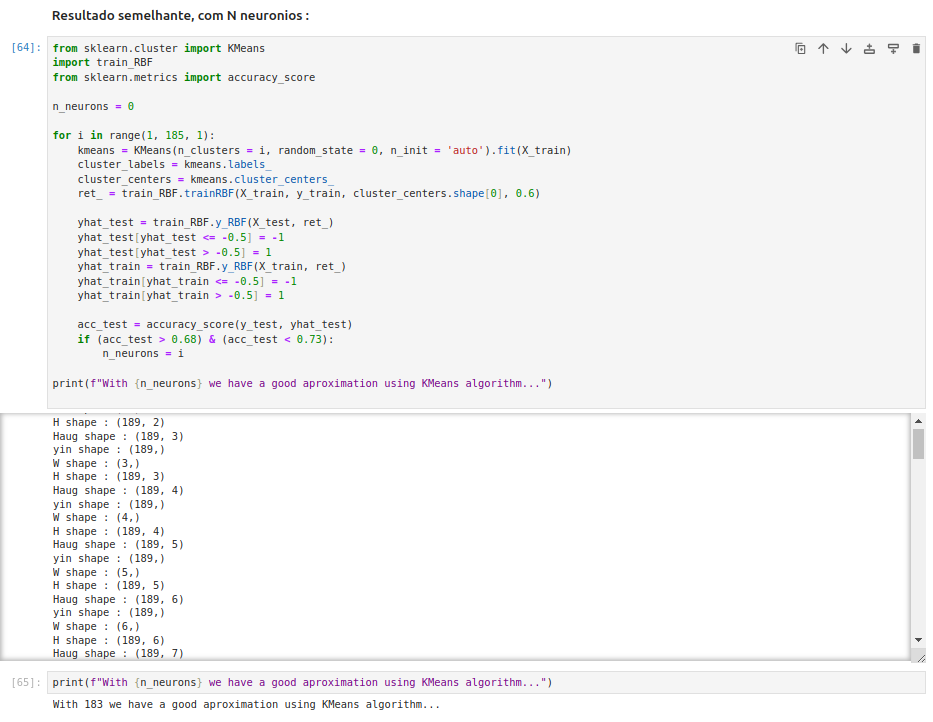
\includegraphics[height=2.5in]{/home/arthur/Desktop/RNA_BRAGA/ex08/statlog_equivalent.png}
                
\end{center}

Como pode ser observado acima, serão necessários 183 neurônios na camada intermediária de uma rede RBF usando o algoritmo KMeans.


\subsection{Breast Cancer}

\vspace{10pt}

\begin{center}

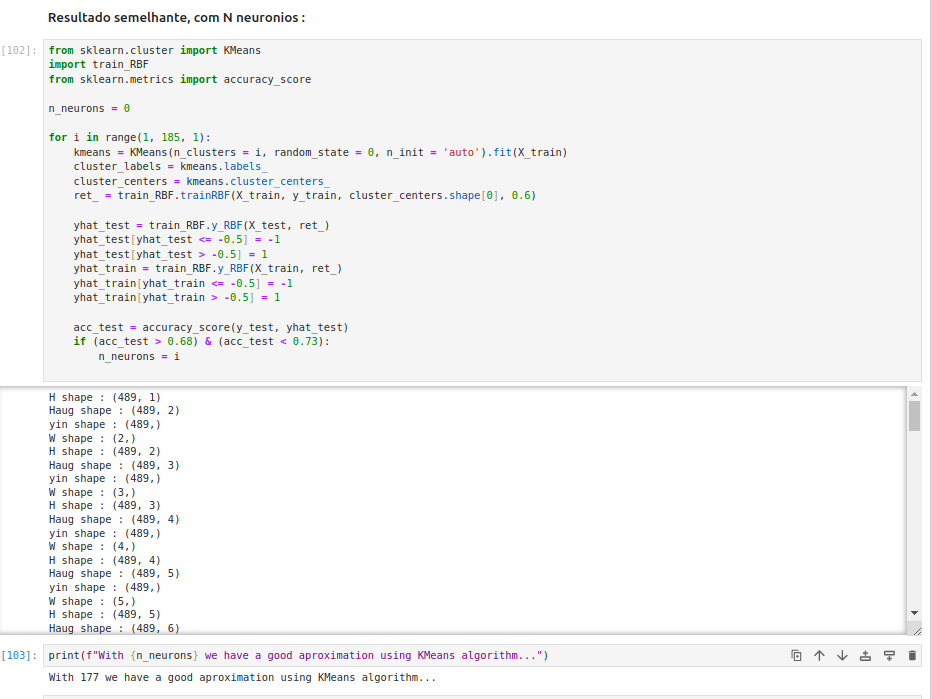
\includegraphics[height=2.5in]{/home/arthur/Desktop/RNA_BRAGA/ex08/BreastCancer_equivalent.png}
                
\end{center}

Como pode ser observado acima, serão necessários 177 neurônios na camada intermediária de uma rede RBF usando o algoritmo KMeans.


\end{document}